% 2018 全国Ⅲ卷文科/理科第19题矩形与半圆弧折叠立体几何示意图
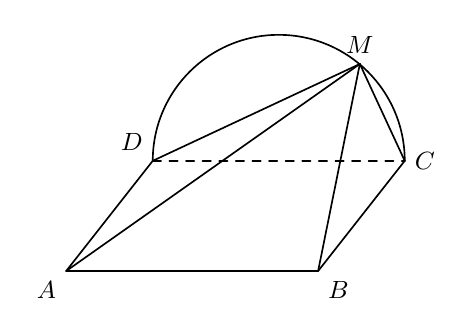
\begin{tikzpicture}[line cap=round, line join=round, line width=0.6pt, font=\small]
  % 矩形顶点坐标
  \coordinate (A) at (0, 0);
  \coordinate (B) at (3.2, 0);
  \coordinate (D) at (1.1, 1.4);
  \coordinate (C) at (4.3, 1.4);
  \coordinate (Ocd) at (2.7, 1.4); % CD中点兼半圆圆心

  % 半圆弧及点M（取圆周角约50度）
  % 半圆直径CD长度为 3.2，半径为 1.6
  \coordinate (M) at (3.73, 2.63);

  % 绘制半圆弧（自C到D）
  \draw (C) arc (0:180:1.6);

  % 矩形底面边：AB, BC, AD为实线，后边CD为虚线
  \draw (A) -- (B) -- (C);
  \draw (A) -- (D);
  \draw[dashed] (D) -- (C);

  % 点M连接各顶点
  \draw (M) -- (D);
  \draw (M) -- (C);
  \draw (M) -- (A);
  \draw (M) -- (B);

  % 顶点标注
  \node[below left] at (A) {$A$};
  \node[below right] at (B) {$B$};
  \node[right] at (C) {$C$};
  \node[above left] at (D) {$D$};
  \node[above] at (M) {$M$};
\end{tikzpicture}
